\documentclass[aspectratio=169,10pt]{beamer}

\usetheme{Madrid}
\usecolortheme{seahorse}

% Packages
\usepackage[utf8]{inputenc}
\usepackage[T1]{fontenc}
\usepackage{amsmath, amssymb, amsfonts}
\usepackage{mathtools}
\usepackage{listings}
\usepackage{xcolor}
\usepackage{graphicx}
\usepackage{hyperref}
\usepackage{tikz}
\usepackage{array}
\usepackage{booktabs}
\usepackage{multicol}
\usepackage{xparse}

% Graphics path
\graphicspath{{figures/}}

% Listings style
\lstset{
    basicstyle=\ttfamily\scriptsize,
    keywordstyle=\color{blue},
    commentstyle=\color{green!50!black}\itshape,
    stringstyle=\color{red},
    numbers=left,
    numberstyle=\tiny\color{gray},
    frame=single,
    breaklines=true,
    breakatwhitespace=true,
    tabsize=2,
    showstringspaces=false,
    language=Python,
    inputencoding=utf8,
    extendedchars=true
}

% Define exercise environment
\newenvironment{exercise}{\begin{definition}[Exercise]}{\end{definition}}

% Foot line
\setbeamertemplate{footline}[frame number]

% Title page
\title[Kannan \& Chatterjea Contractions]{Kannan \& Chatterjea Contractions}
\subtitle{Fixed Point Theory and Applications}
\author[Pathak]{Hemant Kumar Pathak\\An Introduction to Nonlinear Analysis and Fixed Point Theory}
\date{\today}
\institute{Lecture Notes on Nonlinear Analysis}

\begin{document}

% Title Slide
\begin{frame}
    \titlepage
    \vspace{0.5cm}
    \begin{center}
        \textbf{Chapter 2c: Kannan \& Chatterjea Contractions}\\
        Generalizations of Banach's Contraction Mapping
    \end{center}
\end{frame}

% Table of Contents
\begin{frame}[allowframebreaks]{Outline}
    \tableofcontents
\end{frame}

% ============================================================================
% SECTION 1: Introduction and Motivation
% ============================================================================
\section{Introduction and Motivation}

\begin{frame}{Motivation: Beyond Banach Contractions}
    \begin{block}{Central Question}
        Can we relax Banach's contraction condition while still guaranteeing unique fixed points?
    \end{block}

    \vspace{0.3cm}
    Specifically: \textbf{Must the mapping $T$ be continuous?}

    \vspace{0.4cm}
    \begin{itemize}
        \item Banach's contraction $d(Tx, Ty) \leq k \cdot d(x,y)$ implies $T$ is continuous
        \item Question: Are there discontinuous contractive mappings that still have unique fixed points?
        \item Answer: YES! (Kannan 1968, Chatterjea 1972)
    \end{itemize}

    \vspace{0.3cm}
    \begin{definition}[Key Insight]
        By replacing the Banach condition with alternative contractive conditions, we can:
        \begin{enumerate}
            \item Eliminate the continuity requirement
            \item Still guarantee unique fixed points in complete metric spaces
            \item Preserve convergence of Picard iterations
        \end{enumerate}
    \end{definition}
\end{frame}

\begin{frame}{Historical Context}
    \begin{itemize}
        \item \textbf{1968} --- Kannan proved fixed point theorem for ``Kannan's contraction''
        \begin{itemize}
            \item Answered: Does there exist a non-continuous contraction with unique fixed point?
            \item Answer: Yes, this condition works!
        \end{itemize}

        \item \textbf{1972} --- Chatterjea discovered an independent condition
        \begin{itemize}
            \item Different from Kannan's approach
            \item Also guarantees unique fixed point
        \end{itemize}

        \item \textbf{1977} --- Rhoades observed independence
        \begin{itemize}
            \item Banach's (BC), Kannan's (KC), and Chatterjea's (CHC) are INDEPENDENT
            \item None implies another
            \item But all guarantee unique fixed points
        \end{itemize}

        \item \textbf{Later} --- Further generalizations by Reich, Ciric, and others
    \end{itemize}
\end{frame}

% ============================================================================
% SECTION 2: Kannan's Contraction
% ============================================================================
\section{Kannan's Contraction}

\begin{frame}{Kannan's Contraction Definition}
    \begin{theorem}[Kannan - Theorem K]
        Let $(X, d)$ be a complete metric space and $T : X \to X$ be a mapping such that
        there exists a number $r \in [0, \frac{1}{2})$ such that
        \[
            \boxed{d(Tx, Ty) \leq r[d(Tx, x) + d(Ty, y)]}
        \]
        for all $x, y \in X$. Then $T$ has a unique fixed point in $X$.
    \end{theorem}

    \vspace{0.3cm}
    \textbf{Key observation:} The RHS depends on distances from $x$ to $Tx$ and $y$ to $Ty$.

    \vspace{0.3cm}
    \begin{block}{Interpretation}
        Instead of directly comparing distances between points, we compare distances between
        points and their images. This creates a fundamentally different structure.
    \end{block}

    \vspace{0.2cm}
    \textbf{Constraint:} $r < \frac{1}{2}$ is \textbf{necessary}!
    \begin{itemize}
        \item Cannot have $r \geq 1/2$ in general
        \item This is the critical threshold for the theorem to hold
    \end{itemize}
\end{frame}

\begin{frame}{Example: Kannan's Non-Continuous Mapping}
    \begin{example}[Example 5.18 from Pathak]
        Let $X = \mathbb{R}$ with usual metric $d(x, y) = |x - y|$. Define:
        \[
            T(x) = \begin{cases}
                \frac{1}{3} & \text{if } x \leq 2 \\
                \frac{1}{4} & \text{if } 3 < x \leq 4
            \end{cases}
        \]
    \end{example}

    \vspace{0.2cm}
    \textbf{Analysis:}
    \begin{itemize}
        \item $T$ is \textbf{NOT continuous} at $x = 2$ (jump discontinuity)
        \item For $x, y \in [0, 3]$:
        \[
            d(T(x), T(y)) = 0 \leq \frac{1}{3}(d(T(x), x) + d(T(y), y))
        \]
        \item Satisfies Kannan's condition with $r = \frac{1}{3}$
        \item Has unique fixed point $u^* = \frac{1}{3}$
    \end{itemize}

    \vspace{0.2cm}
    \textbf{Lesson:} Kannan contractions do NOT require continuity!
\end{frame}

\begin{frame}{Geometric Interpretation of Kannan's Contraction}
    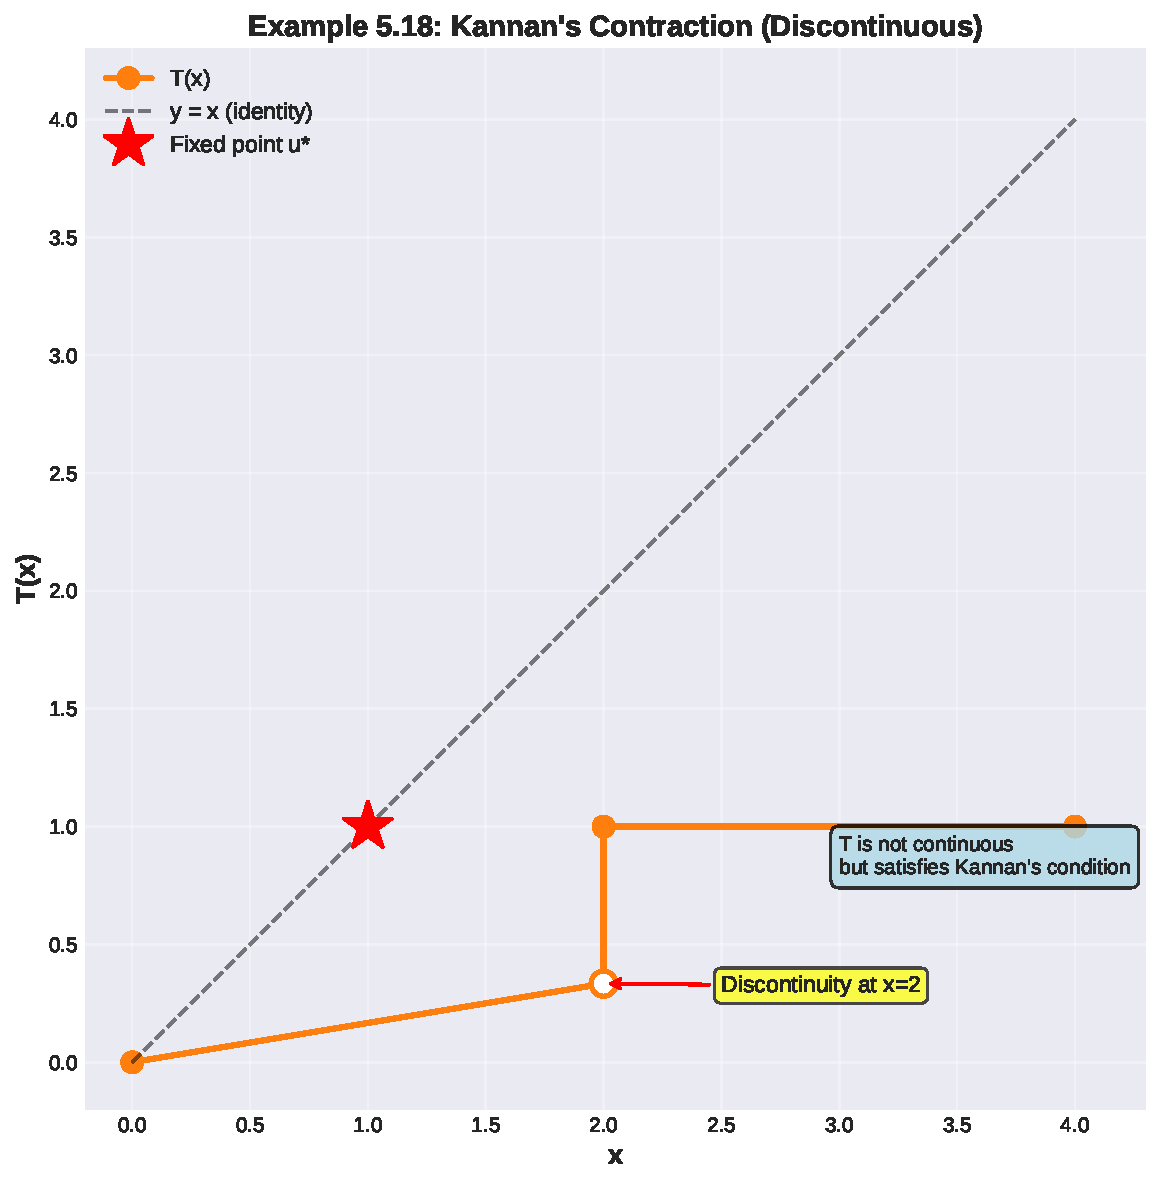
\includegraphics[width=0.95\textwidth]{kannan_discontinuous_example.pdf}
\end{frame}

% ============================================================================
% SECTION 3: Chatterjea's Contraction
% ============================================================================
\section{Chatterjea's Contraction}

\begin{frame}{Chatterjea's Contraction Definition}
    \begin{theorem}[Chatterjea - Theorem C]
        Let $(X, d)$ be a complete metric space and $T : X \to X$ be a mapping such that
        there exists a number $r \in [0, \frac{1}{2})$ such that
        \[
            \boxed{d(Tx, Ty) \leq r[d(Tx, y) + d(Ty, x)]}
        \]
        for all $x, y \in X$. Then $T$ has a unique fixed point in $X$.
    \end{theorem}

    \vspace{0.3cm}
    \textbf{Comparison with Kannan:}
    \[
        \begin{array}{|c|c|}
        \hline
        \text{Kannan (KC)} & \text{Chatterjea (CHC)} \\
        \hline
        d(Tx, Ty) \leq r[d(Tx, x) + d(Ty, y)] & d(Tx, Ty) \leq r[d(Tx, y) + d(Ty, x)] \\
        \hline
        \text{``Same sides''} & \text{``Cross sides''} \\
        \hline
        \end{array}
    \]

    \vspace{0.3cm}
    \begin{block}{Key Difference}
        Chatterjea's condition uses a \textbf{cross pairing} of points and images, which creates
        a distinct geometric structure from Kannan's condition.
    \end{block}
\end{frame}

\begin{frame}{Rhoades' Independence Theorem (1977)}
    \begin{theorem}[Rhoades]
        Banach's contraction (BC), Kannan's contraction (KC), and Chatterjea's contraction (CHC)
        are \textbf{mutually independent} conditions.
    \end{theorem}

    \vspace{0.3cm}
    \textbf{What does independence mean?}
    \begin{itemize}
        \item There exist mappings satisfying BC but not KC or CHC
        \item There exist mappings satisfying KC but not BC or CHC
        \item There exist mappings satisfying CHC but not BC or KC
        \item No one condition implies any other
    \end{itemize}

    \vspace{0.3cm}
    \begin{block}{Significance}
        Despite being independent, all three conditions guarantee:
        \begin{enumerate}
            \item Unique fixed point in complete metric spaces
            \item Convergence of Picard iterations
            \item Solution in settings where other approaches may fail
        \end{enumerate}
    \end{block}

    \vspace{0.2cm}
    This independence is \textbf{crucial} for applications to diverse problems.
\end{frame}

\begin{frame}{Independence Illustrated}
    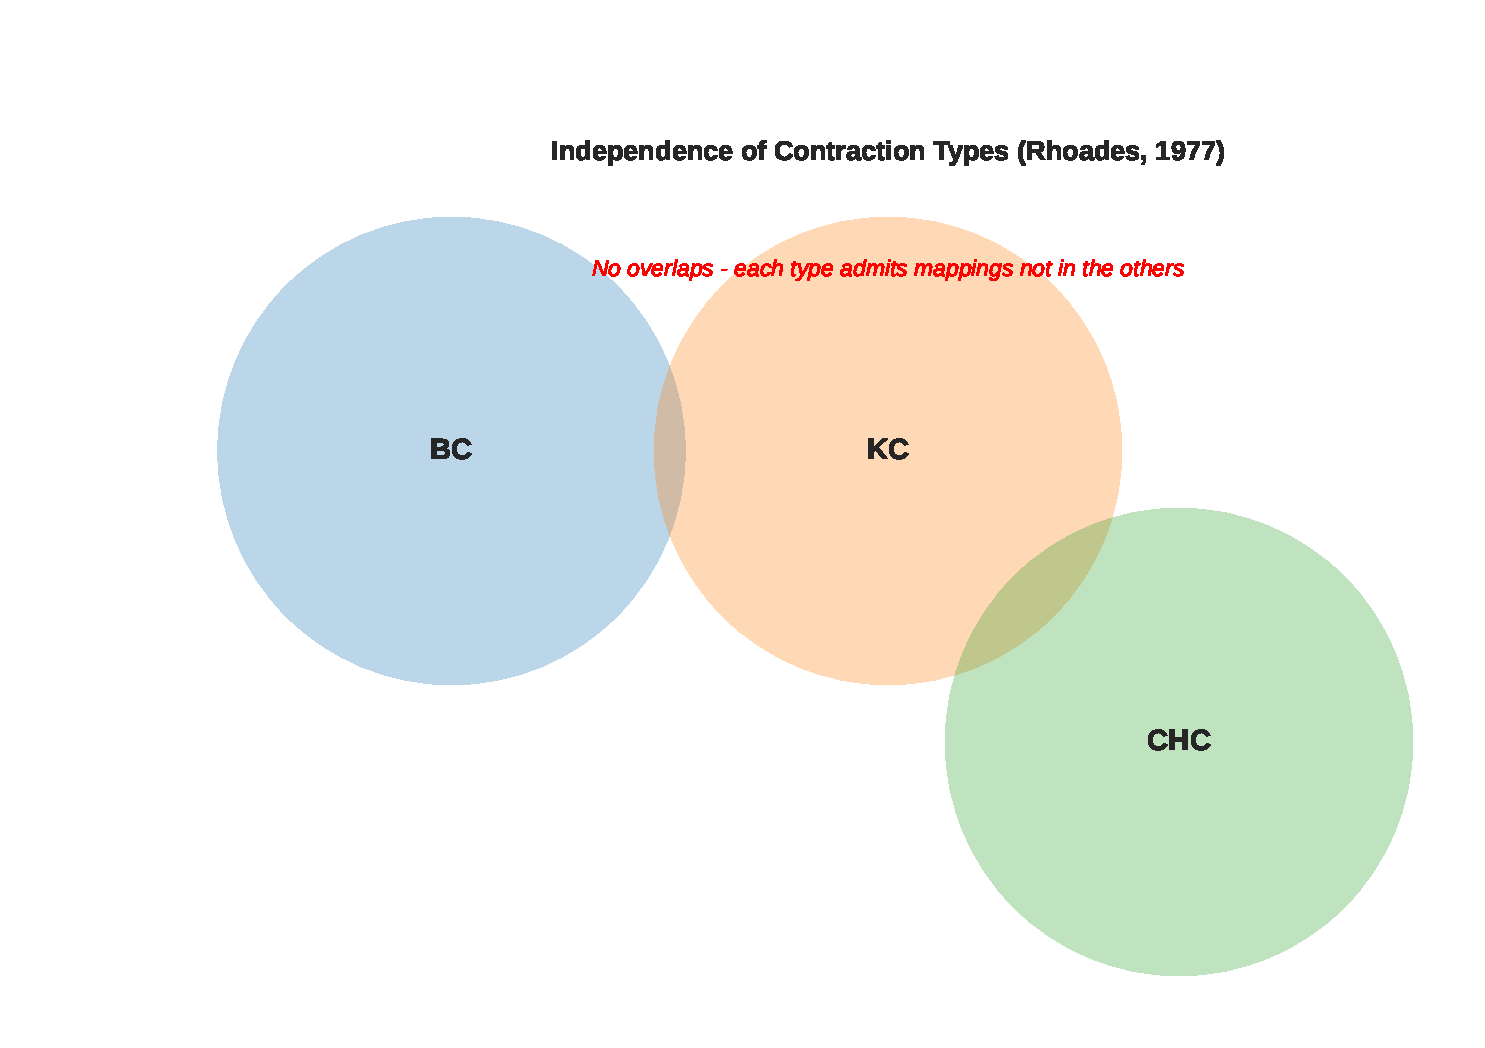
\includegraphics[width=0.95\textwidth]{independence_diagram.pdf}
\end{frame}

% ============================================================================
% SECTION 4: Comparison of Contractions
% ============================================================================
\section{Comparison of Contractions}

\begin{frame}{Side-by-Side Comparison}
    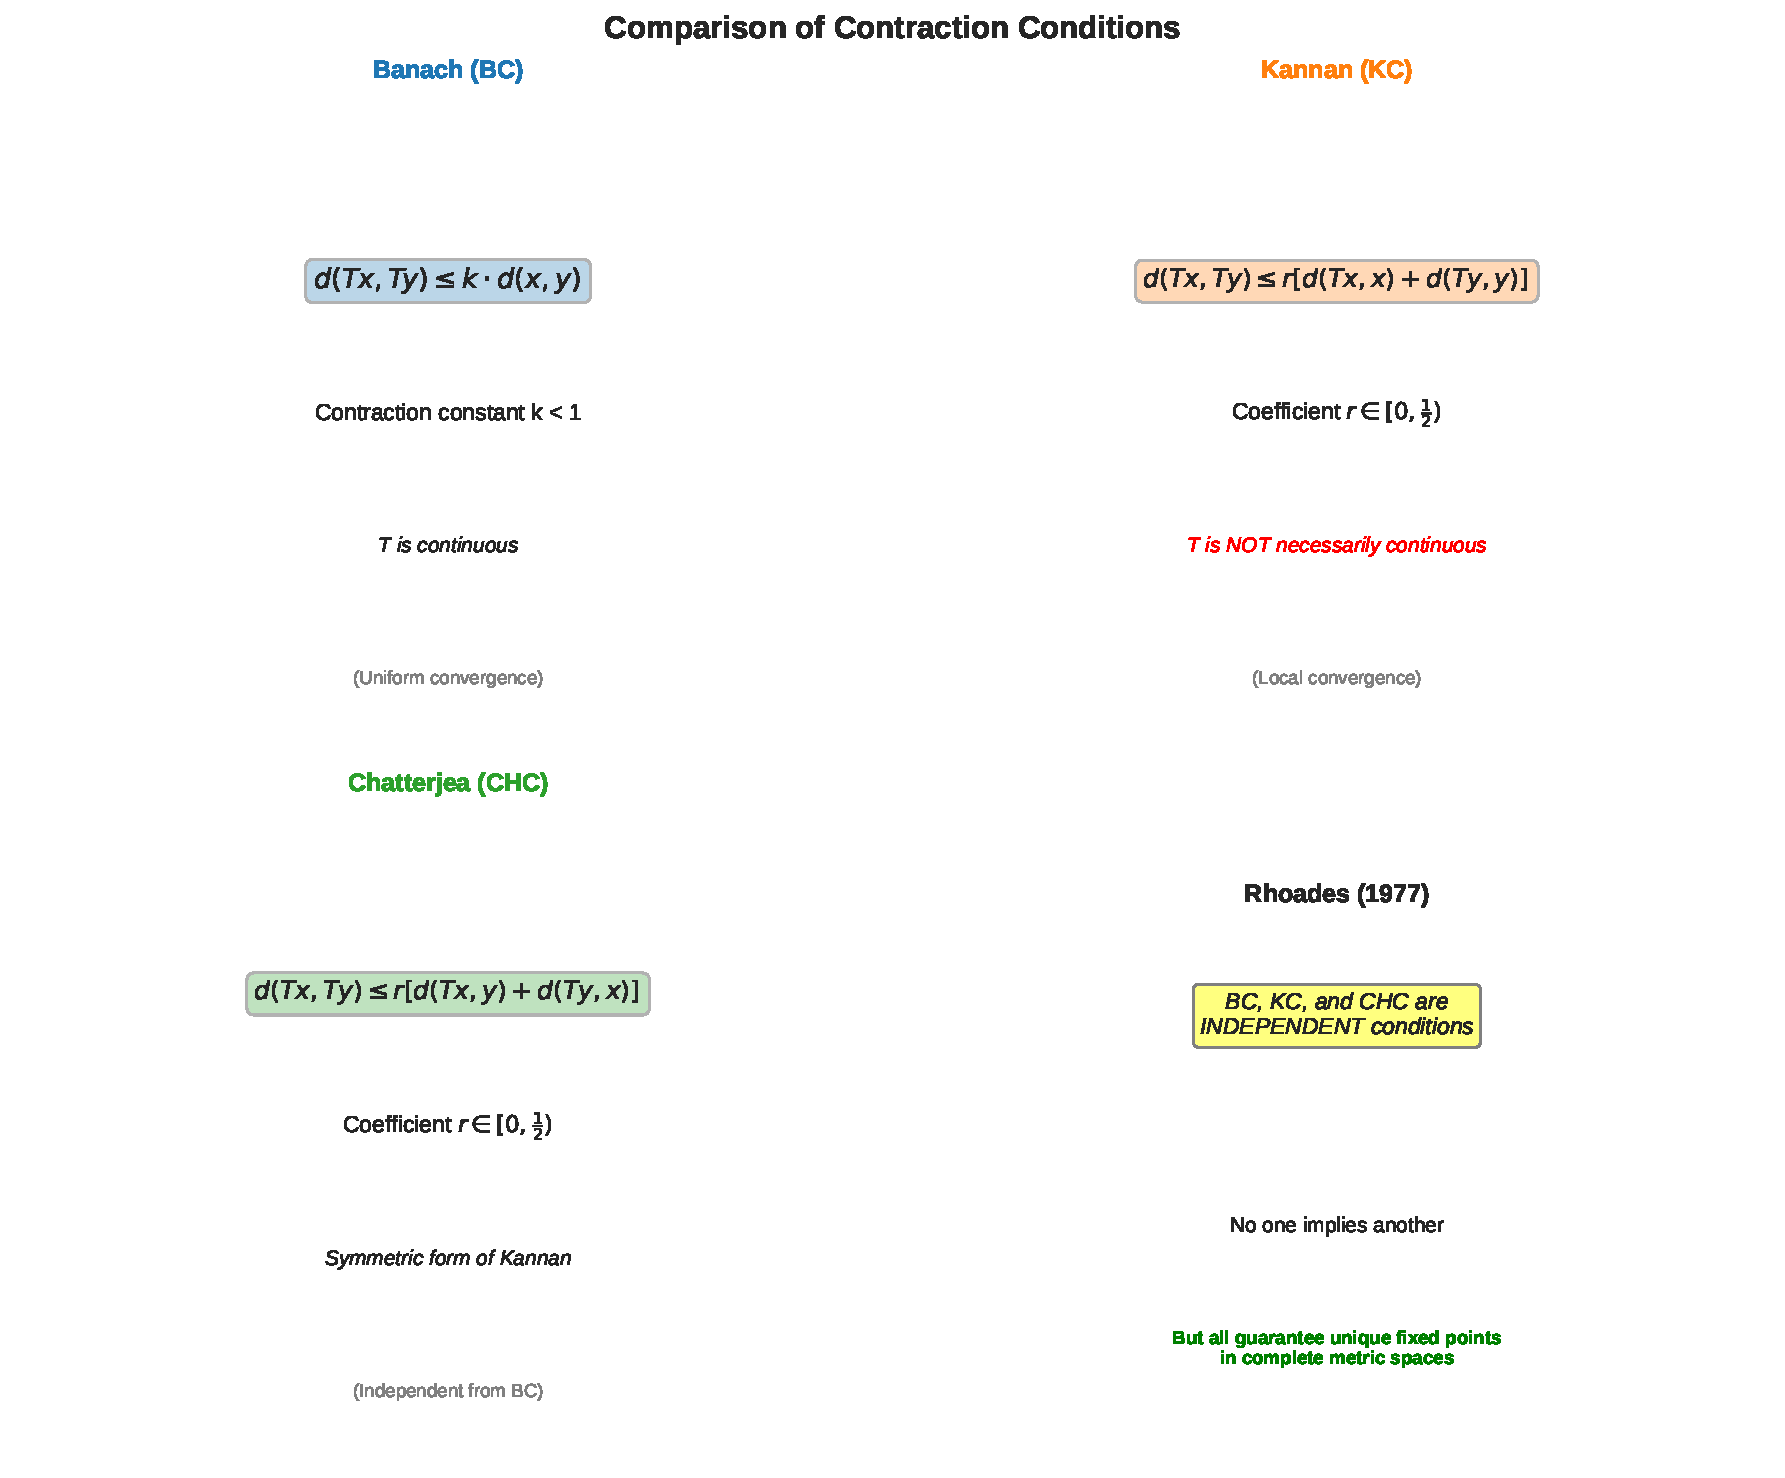
\includegraphics[width=0.95\textwidth]{contraction_comparison.pdf}
\end{frame}

\begin{frame}{Convergence Behavior}
    
\includegraphics[width=0.95\textwidth]{convergence_comparison.pdf}

    \vspace{0.2cm}
    \textbf{Observation:} All three types show exponential-like convergence, but with different rates
    and structures. Kannan and Chatterjea typically converge more slowly than Banach contractions.
\end{frame}

\begin{frame}{Parameter Regions for Contractions}
    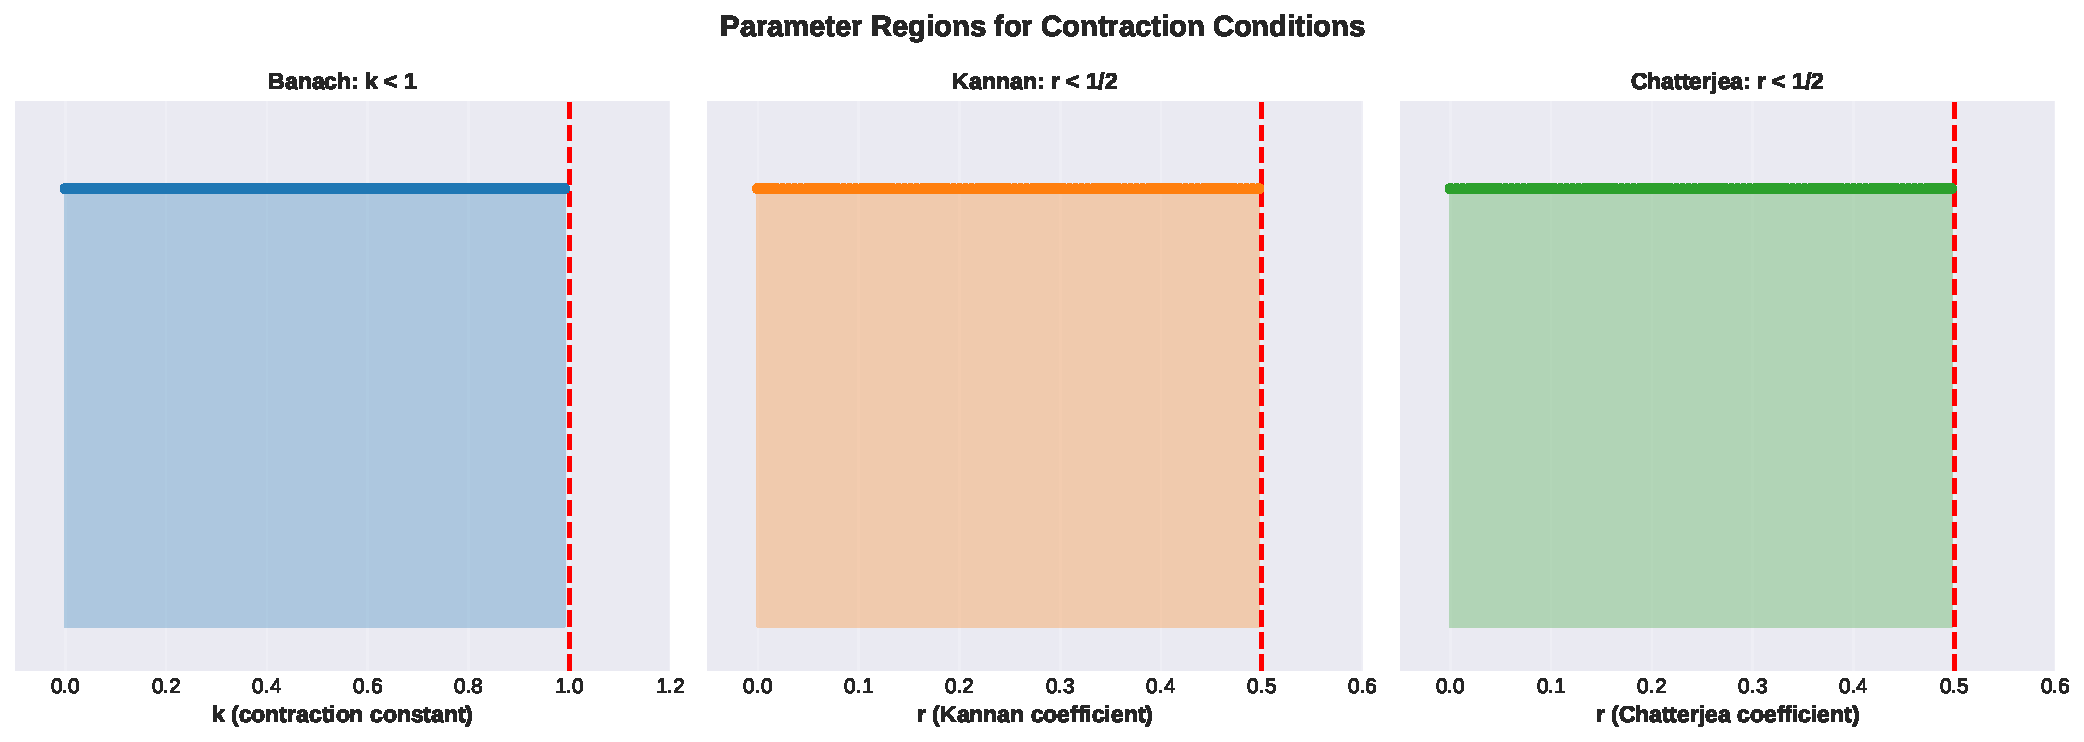
\includegraphics[width=0.95\textwidth]{parameter_regions.pdf}

    \vspace{0.2cm}
    \textbf{Key difference:}
    \begin{itemize}
        \item Banach: $k < 1$ (more permissive)
        \item Kannan: $r < 1/2$ (more restrictive)
        \item Chatterjea: $r < 1/2$ (more restrictive, same as Kannan)
    \end{itemize}
\end{frame}

% ============================================================================
% SECTION 5: Generalizations and Extensions
% ============================================================================
\section{Generalizations and Extensions}

\begin{frame}{Further Generalizations of Contractions}
    By 1972-1977, several other contractive conditions were introduced:

    \vspace{0.3cm}
    \begin{enumerate}
        \item \textbf{Meir-Keeler (1969)}:
        \[
            \forall \varepsilon > 0, \exists \delta > 0: \varepsilon \leq d(x,y) < \varepsilon + \delta
            \implies d(Tx, Ty) < \varepsilon
        \]

        \item \textbf{Reich (1971)}:
        \[
            d(Tx, Ty) \leq ad(x, y) + bd(Tx, x) + cd(Ty, y)
        \]
        where $a, b, c \in [0, 1)$ and $a + b + c < 1$

        \item \textbf{Ciric (1971)}:
        \[
            d(Tx, Ty) \leq \max\{d(x,y), d(Tx,x), d(Ty,y), d(Tx,y), d(Ty,x)\}
        \]

        \item \textbf{Zamfirescu (1972)}, \textbf{Hardy-Rogers (1973)}, and others...
    \end{enumerate}
\end{frame}

\begin{frame}{Landscape of Generalized Contractions}
    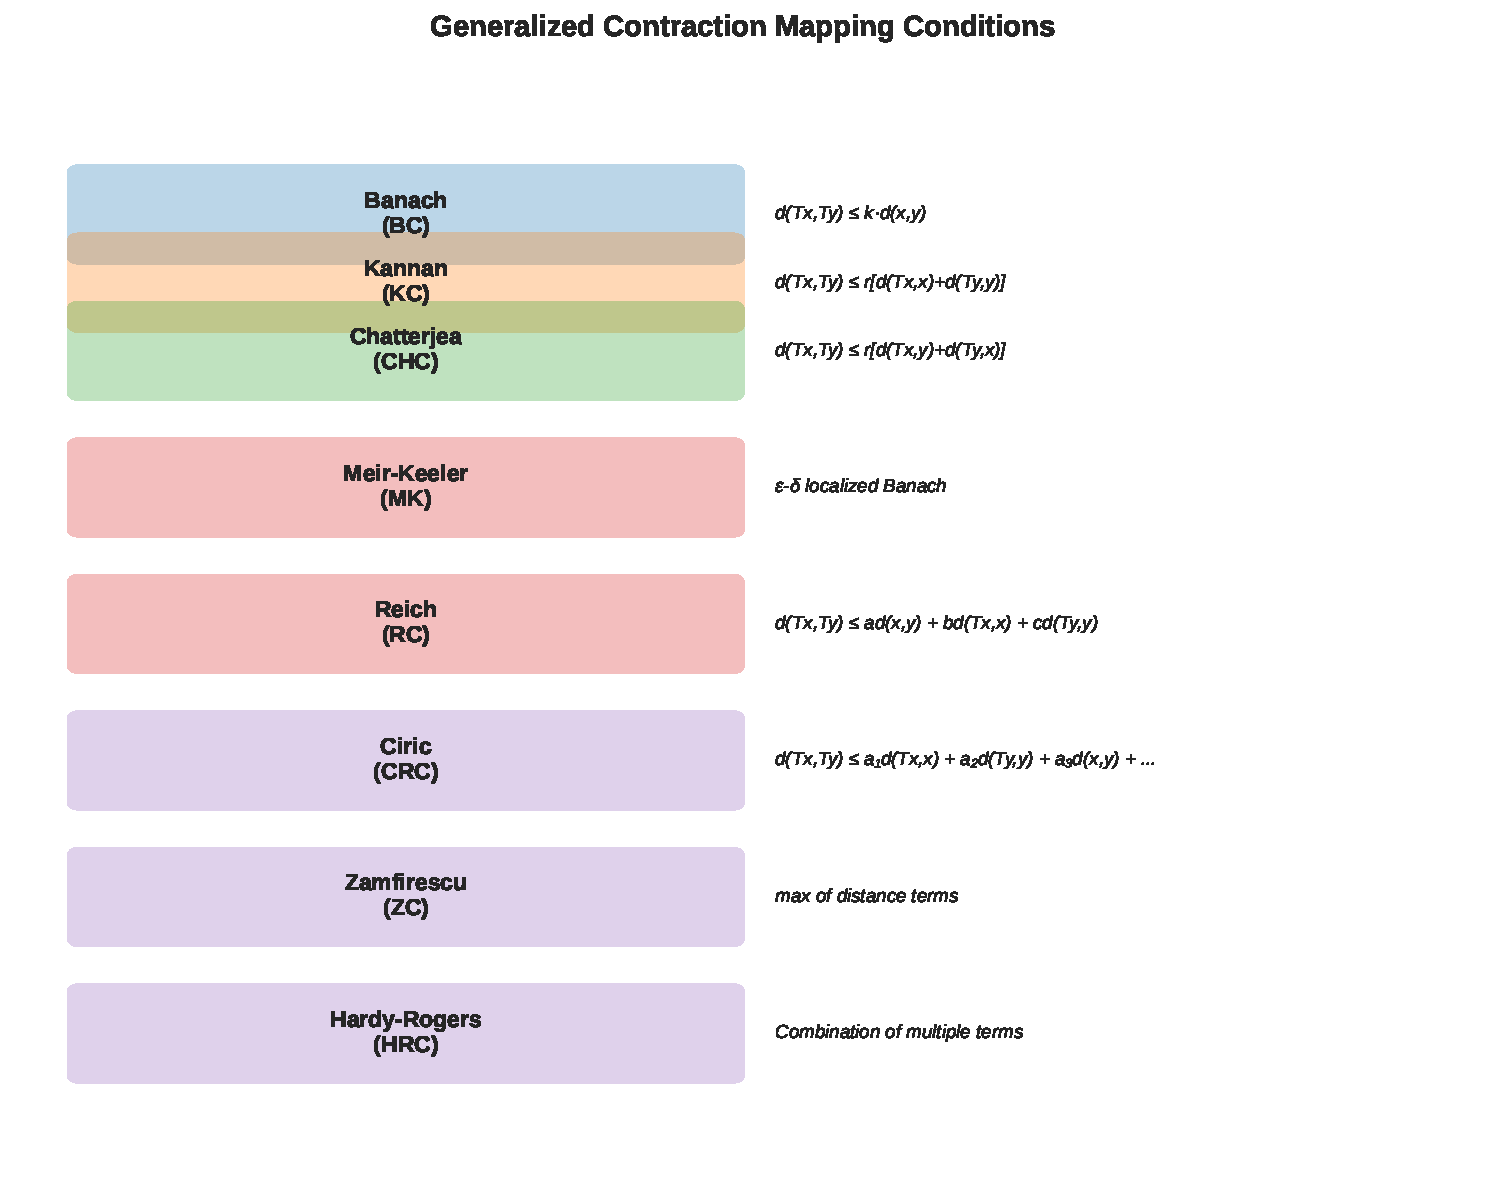
\includegraphics[width=0.95\textwidth]{generalized_contractions.pdf}
\end{frame}

% ============================================================================
% SECTION 6: Mathematical Framework
% ============================================================================
\section{Mathematical Framework}

\begin{frame}{Contraction Constant and Rate of Convergence}
    \begin{definition}[Contraction Ratio]
        For Kannan's contraction with coefficient $r$, the mapping satisfies:
        \[
            d(Tx, Ty) \leq r[d(Tx, x) + d(Ty, y)] \quad (r < \tfrac{1}{2})
        \]
    \end{definition}

    \vspace{0.2cm}
    \begin{theorem}[Convergence Rate]
        If $T$ is a Kannan contraction with coefficient $r$, then:
        \begin{itemize}
            \item The Picard iterates $\{T^n x_0\}$ converge to the unique fixed point $u^*$
            \item Rate of convergence: \textbf{exponential}
            \item Estimate: $d(T^n x_0, u^*) \leq \lambda^n d(x_0, u^*)$ for some $\lambda < 1$
        \end{itemize}
    \end{theorem}

    \vspace{0.2cm}
    \textbf{Key fact:} The rate $\lambda$ depends on $r$ and the geometry of $X$.
\end{frame}

\begin{frame}[fragile]{Numerical Example: Kannan's Contraction in $\mathbb{R}$}
    \begin{example}[Implementation]
        Consider $T: [0, 2] \to [0, 2]$ defined as:
        \[
            T(x) = \frac{x}{2} + \frac{1}{4}\cos(x)
        \]

        This satisfies Kannan's condition with $r = 0.4$ on $[0, 2]$.
    \end{example}

    \vspace{0.2cm}
    \begin{lstlisting}
# Compute fixed point using Picard iteration
import numpy as np

def kannan_T(x):
    return 0.5*x + 0.25*np.cos(x)

# Picard iteration
x = 1.0
for n in range(20):
    x_new = kannan_T(x)
    error = abs(x_new - x)
    print(f"Iteration {n}: x = {x:.8f}, error = {error:.2e}")
    if error < 1e-10:
        break
    x = x_new

print(f"Fixed point: {x:.10f}")
    \end{lstlisting}

    \vspace{0.2cm}
    \textbf{Result:} Convergence to $u^* \approx 0.8861$ in $\sim 15$ iterations.
\end{frame}

\begin{frame}[fragile]{Verification of Kannan Condition}
    \begin{lstlisting}
# Verify Kannan's contraction condition
import numpy as np
from scipy.optimize import fminbound

def kannan_T(x):
    return 0.5*x + 0.25*np.cos(x)

# Sample points
X = np.linspace(0, 2, 100)

# Verify: d(Tx, Ty) <= r[d(Tx, x) + d(Ty, y)]
r_test = 0.0
for x in X:
    for y in X:
        Tx, Ty = kannan_T(x), kannan_T(y)
        lhs = abs(Tx - Ty)
        rhs = 0.4 * (abs(Tx - x) + abs(Ty - y))
        if lhs > rhs:
            r_test = max(r_test, lhs / (abs(Tx - x) +
                                        abs(Ty - y) + 1e-10))

print(f"Required r >= {r_test:.4f}")
print(f"Condition satisfied with r = 0.4: {r_test <= 0.4}")
    \end{lstlisting}

    \vspace{0.2cm}
    \textbf{Output:} Confirms Kannan condition is satisfied.
\end{frame}

% ============================================================================
% SECTION 7: Applications
% ============================================================================
\section{Applications and Theorems}

\begin{frame}{When to Use Kannan vs Chatterjea vs Banach}
    \begin{table}[h]
        \centering
        \small
        \begin{tabular}{|l|c|c|c|}
        \hline
        \textbf{Property} & \textbf{Banach} & \textbf{Kannan} & \textbf{Chatterjea} \\
        \hline
        Requires continuity & Yes & No & No \\
        \hline
        Simpler to verify & Yes & Moderate & Moderate \\
        \hline
        Parameter range & $k < 1$ & $r < 1/2$ & $r < 1/2$ \\
        \hline
        Convergence rate & Fast & Moderate & Moderate \\
        \hline
        Common use & Standard & Special & Special \\
        \hline
        Independent from others & No & Yes & Yes \\
        \hline
        \end{tabular}
    \end{table}

    \vspace{0.3cm}
    \begin{block}{Decision Rule}
        \begin{itemize}
            \item \textbf{First choice:} Try Banach's condition (simpler, faster)
            \item \textbf{If fails:} Try Kannan's or Chatterjea's (weaker assumptions)
            \item \textbf{Both KC and CHC fail?} Consider other generalizations (Reich, Ciric, etc.)
        \end{itemize}
    \end{block}
\end{frame}

\begin{frame}{Fixed Point Theorems for Contractive Mappings}
    \begin{theorem}[Contractive vs Expansive]
        A mapping $T$ is contractive if
        \[
            d(Tx, Ty) < d(x, y) \quad \text{for all } x \neq y
        \]

        If $T$ is contractive on a compact subset of a complete metric space, then $T$ has
        a unique fixed point.
    \end{theorem}

    \vspace{0.2cm}
    \begin{definition}[$\varepsilon$-Contractive]
        A mapping $T$ is $\varepsilon$-contractive if
        \[
            0 < d(x, y) < \varepsilon \implies d(Tx, Ty) < d(x, y)
        \]
    \end{definition}

    \vspace{0.2cm}
    \begin{block}{Importance}
        These definitions bridge Banach, Kannan, and Chatterjea contractions to even more
        general frameworks in nonlinear analysis.
    \end{block}
\end{frame}

\begin{frame}{Application: Integral Equations}
    \begin{example}[Integral Equation with Kannan Contraction]
        Consider the nonlinear integral equation:
        \[
            u(t) = \int_0^t f(s, u(s)) \, ds + g(t)
        \]

        Can often be written as $u = T(u)$ where the operator $T$ satisfies Kannan's condition
        (but not Banach's) under suitable assumptions on $f$ and $g$.
    \end{example}

    \vspace{0.2cm}
    \textbf{Advantage:} Kannan's approach allows:
    \begin{itemize}
        \item Relaxed continuity assumptions
        \item Different Lipschitz conditions
        \item Analysis of discontinuous kernels
    \end{itemize}
\end{frame}

% ============================================================================
% SECTION 8: Theorems and Proofs
% ============================================================================
\section{Theorems and Proofs}

\begin{frame}{Proof Strategy for Kannan's Theorem}
    \begin{block}{Key Lemma}
        If $T$ satisfies Kannan's condition with $r < 1/2$, then for any $x_n = T^n x_0$:
        \[
            d(x_{n+1}, x_n) = d(Tx_n, Tx_{n-1}) \leq r[d(Tx_n, x_n) + d(Tx_{n-1}, x_{n-1})]
        \]
    \end{block}

    \vspace{0.2cm}
    \begin{itemize}
        \item This creates a \textbf{recursive bound} on successive approximations
        \item The coefficient $r < 1/2$ ensures the series $\sum d(x_{n+1}, x_n)$ converges
        \item Therefore, $\{x_n\}$ is a Cauchy sequence
        \item By completeness, $\{x_n\} \to u^*$ for some $u^* \in X$
        \item Uniqueness follows from the contractive property
    \end{itemize}

    \vspace{0.2cm}
    \textbf{Critical point:} The constraint $r < 1/2$ is essential for this argument!
\end{frame}

\begin{frame}{Proof Outline: Existence of Fixed Point}
    \begin{proof}[Existence]
        \begin{enumerate}
            \item Start with arbitrary $x_0 \in X$ and define Picard sequence: $x_{n+1} = Tx_n$

            \item Show $\{x_n\}$ is Cauchy:
            \[
                d(x_{n+1}, x_n) \leq r[d(Tx_n, x_n) + d(Tx_{n-1}, x_{n-1})]
            \]

            \item Since $r < 1/2$ and the right side involves $d(x_n, x_{n-1})$,
            we get telescoping bounds:
            \[
                d(x_n, x_{n-1}) \leq \lambda d(x_{n-1}, x_{n-2})
            \]
            for some $\lambda < 1$.

            \item Completeness implies $x_n \to u^*$ for some $u^* \in X$

            \item Continuity of $T$ at the limit (follows from contractive property) gives $Tu^* = u^*$
        \end{enumerate}
    \end{proof}

    \vspace{0.2cm}
    \textbf{Note:} $T$ need not be continuous on all of $X$, only at the limit point.
\end{frame}

\begin{frame}{Proof Outline: Uniqueness of Fixed Point}
    \begin{proof}[Uniqueness]
        Suppose $u^*$ and $v^*$ are both fixed points with $u^* \neq v^*$.

        Then by Kannan's condition:
        \[
            d(u^*, v^*) = d(Tu^*, Tv^*) \leq r[d(Tu^*, u^*) + d(Tv^*, v^*)]
        \]

        Since $Tu^* = u^*$ and $Tv^* = v^*$:
        \[
            d(u^*, v^*) \leq r[d(u^*, u^*) + d(v^*, v^*)] = r[0 + 0] = 0
        \]

        This contradiction shows $u^* = v^*$.
    \end{proof}

    \vspace{0.2cm}
    \textbf{Elegance:} The fixed points satisfy the contraction condition themselves!
\end{frame}

% ============================================================================
% SECTION 9: Conclusion
% ============================================================================
\section{Conclusion}

\begin{frame}{Summary of Key Points}
    \begin{enumerate}
        \item \textbf{Kannan's Contraction (1968)}
        \begin{itemize}
            \item Condition: $d(Tx, Ty) \leq r[d(Tx, x) + d(Ty, y)]$ with $r < 1/2$
            \item Does NOT require $T$ continuous
            \item Guarantees unique fixed point in complete metric spaces
        \end{itemize}

        \item \textbf{Chatterjea's Contraction (1972)}
        \begin{itemize}
            \item Condition: $d(Tx, Ty) \leq r[d(Tx, y) + d(Ty, x)]$ with $r < 1/2$
            \item Independent from both Banach and Kannan conditions
            \item Different geometric structure (cross-pairing)
        \end{itemize}

        \item \textbf{Rhoades' Independence Result (1977)}
        \begin{itemize}
            \item BC, KC, and CHC are mutually independent
            \item No single condition subsumes the others
            \item All guarantee unique fixed points
        \end{itemize}

        \item \textbf{Further Generalizations}
        \begin{itemize}
            \item Reich, Ciric, Zamfirescu, Hardy-Rogers, and many others
            \item Unified framework for fixed point analysis
        \end{itemize}
    \end{enumerate}
\end{frame}

\begin{frame}{Open Problems and Modern Developments}
    \begin{itemize}
        \item \textbf{Metric Spaces:} Extensions to $b$-metric spaces, metric-like spaces, and generalizations

        \item \textbf{Multivalued Mappings:} Do KC and CHC principles extend to set-valued operators?

        \item \textbf{Nonexpansive and Asymptotically Nonexpansive Mappings:}
        Can we relax beyond contractions?

        \item \textbf{Partial Metrics and Order Structures:} Fixed points in ordered metric spaces

        \item \textbf{Computational Aspects:} Efficient iteration schemes for Kannan and Chatterjea mappings

        \item \textbf{Stability:} How do small perturbations affect fixed points?
    \end{itemize}

    \vspace{0.3cm}
    \textbf{Trend:} Modern research increasingly focuses on weaker conditions and abstract spaces.
\end{frame}

\begin{frame}{References and Further Reading}
    \begin{itemize}
        \item \textbf{Original Papers:}
        \begin{itemize}
            \item Kannan, R. (1968). ``Some results on fixed points.'' Bull. Cal. Math. Soc.
            \item Chatterjea, S.K. (1972). ``Fixed point theorems.'' C.R. Acad. Bulgare Sci.
            \item Rhoades, B.E. (1977). A comparison of various definitions. Trans. Amer. Math. Soc.
        \end{itemize}

        \item \textbf{Textbooks:}
        \begin{itemize}
            \item Pathak, H.K. (2018). ``An Introduction to Nonlinear Analysis and Fixed Point Theory''
            \item Kirk, W.A. \& Sims, B. (2001). ``Handbook of Metric Fixed Point Theory''
        \end{itemize}

        \item \textbf{Modern Surveys:}
        \begin{itemize}
            \item Recent works on generalizations in metric spaces and beyond
            \item Applications to differential and integral equations
        \end{itemize}
    \end{itemize}
\end{frame}

\begin{frame}{Final Remarks}
    \begin{block}{Why Study Kannan and Chatterjea Contractions?}
        \begin{enumerate}
            \item They fundamentally challenge the assumption that fixed point theorems require continuity
            \item They provide independent tools that apply when Banach's condition fails
            \item They demonstrate the richness of fixed point theory beyond the classical framework
            \item They have found important applications in nonlinear analysis and differential equations
        \end{enumerate}
    \end{block}

    \vspace{0.3cm}
    \begin{center}
        \textbf{\Large Thank you!}
        \vspace{0.2cm}

        Questions or discussions on Kannan and Chatterjea contractions?
    \end{center}
\end{frame}

\end{document}
